\chapter{RESEARCH APPROACH}
\label{research-approach}
\section{PROV-PUB-O: a provenance ontology for research publications}
This section presents the approach to the creation of an ontology for capturing provenance in the process of preparing research publications. The ontology is divided into two parts. 

The first part --- Section~\ref{subsec:structure} --- describes the structure of a research publication. We base our work on the Document Components Ontology (DoCO), which is one of the Semantic Publishing and Referencing Ontologies (SPAR). SPAR focuses a lot on modeling citations and bibliographic references. Four out of the eight ontologies in SPAR deal with citations and bibliographic references. (They are CiTO, the Citation Typing Ontology, FaBiO, the FRBR-aligned Bibliographic Ontology, BiRO, the Bibliographic Reference Ontology, and C4O, the Citation Counting and Context Characterization Ontology.) So SPAR is good for modeling the linkage between publications. 

In this proposal we focus on the reproducibility of a certain publication, so we do not delve deep into citations and bibliographic references as they have nothing to do with the computational experiments presented in the current publication. 

We model the structure of a research publication because experimental results must reside somewhere in the publication. Textual elements in the publication provide contextual information and explanation for the reported results. Although these elements are not parts of the process leading to the reported results, they are documentation that help readers to correctly interpret the results, so we include structural elements of research publications in the provenance.

The second part --- Section~\ref{subsec:process} --- describes the process leading to the reported results. It is a specialization of the W3C Provenance Ontology (PROV-O) for the use case of research publication preparation. We base the development of PROV-PUB-O on PROV-O because using general provenance ontologies such as PROV-O proves to be an effective way to keep track of the lineage of the source data and the changing processes leading to the final results. 

The goal of the specialization is to make the specialized ontology, namely PROV-PUB-O, detailed enough to enable the creation of \emph{executable provenance graphs} (EPGs). In an EPG, the semantics of each element in the process leading to the reported results is well defined, so the replication of the process becomes straightforward. Moreover, the process described with an EPG can even be used to validate the scientific conclusions by allowing readers to adapt the experiment reported in the paper and carry out their own studies.

The hypothesis to justify for PROV-PUB-O is that it is useful in the use case of modeling research publication preparation process in the domain of earth science for the purpose of replicating data transformation processes and validating scientific conclusions. We would like to show that less effort is required to create EPGs with PROV-PUB-O than with PROV-O. We will cover the measurement of effort amount and the details of the benchmark modeling tasks in Section~\ref{subsec:evaluation}.

\subsection{Publication structure modeling}
\label{subsec:structure}
Document structure models such as the Document Components Ontology (DoCO)\footnote{DoCO, the Document Components Ontology: http://purl.org/spar/doco} are usually based on structural patterns \cite{di2014dealing} and rhetorical structure theory (RST) \cite{taboada2006rhetorical}.

Here we take DoCO as an example. DoCO defines structural (e.g. block, inline, paragraph, section, chapter, etc. --- meaning what the component looks like) as well as rhetorical (e.g. introduction, discussion, acknowledgements, reference list, figure, appendix, etc. --- meaning what role the component plays in the document) document components.

Figure~\ref{fig:doco} shows the components of DoCO and the respective classes included in these components.
\begin{figure}[h]
	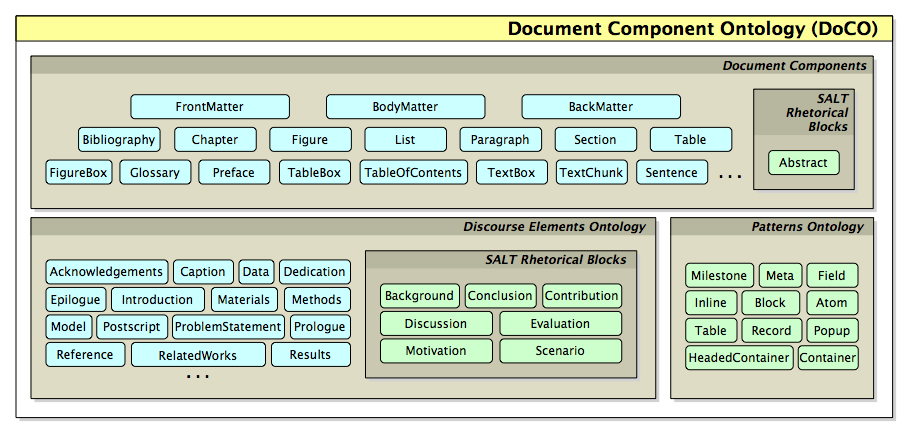
\includegraphics[width=\textwidth]{doco-architecture.png}
	\caption{Architecture of DoCO, the Document Components Ontology}
	\label{fig:doco}
\end{figure}

Structural document component types are closely related to the typesetting of the component contents. For example, if a block of text consisting of a title and several paragraphs is known to be a chapter, then at the time of rendering this block, the title can be made larger, proper font and size can be set for the content paragraphs, and the proper spacing can be set between this block and the blocks previous and next to it. Therefore, each structural document component type is like a class used to label HTML elements, and to be rendered according to class styles defined in Cascading Style Sheets (CSS).

Rhetorical document component types are completely irrelevant to typesetting --- just knowing a block of text is an ``introduction'' has nothing to do with properly formatting it. Rather, rhetorical types focus on the \emph{relations} between document parts, so these types are actually \emph{types of relations}. For example, the ``introduction'' component of a paper is usually a chapter, but theoretically it can be a section or even just a paragraph, leading to very different typesetting options. But just look at how we call this ``introduction'' component -- we call it ``introduction \emph{of} a paper'', i.e., an introduction component is always \emph{of something}. It does not make sense to have a ``floating'' introduction attached to nothing. 

In light of this relational perspective of rhetorical types, we make the following changes from DoCO:

\begin{itemize}
	\item The sro:Abstract class is changed to the pub:abstract property, whose domain is (doco:Chapter or doco:Section) and (dcterms:isPartOf some doco:BodyMatter or doco:FrontMatter), and range is pub:Document. The prefix sro expands to http://salt.semanticauthoring.org/ontologies/sro\# and stands for SALT (Semantically Annotated \LaTeX \cite{groza2007salt}) Rhetorical Ontology. The prefix doco expands to http://purl.org/spar/doco/, and the prefix dcterms expands to http://purl.org/dc/terms/, meaning DCMI (Dublin Core$^{\textregistered}$ Metadata Initiative) Metadata Terms\footnote{DCMI Metadata Terms: http://dublincore.org/documents/dcmi-terms/}. Finally, the prefix pub is for PROV-PUB-O, which is under development and not published yet.
	\item The sro:Background class is changed to the pub:background property, whose domain is (doco:Chapter or doco:Section) and (dcterms:isPartOf some doco:BodyMatter), and range is pub:Document. 
	\item Classes sro:Conclusion, sro:Contribution, sro:Discussion, sro:Evaluation, sro:Motivation, sro:Scenario are changed in the same manner as sro:Background. Note that these classes are different from sro:Abstract in that they cannot be part of the front matter component of a document.
	%\item The class deo:Acknowledgements \comment{not sure yet.} The prefix deo here expands to http://purl.org/spar/deo/ and stands for the Discourse Elements Ontology\footnote{The Discourse Elements Ontology: http://purl.org/spar/deo}.
\end{itemize}

The hypotheses to justify here is that properties are more useful than rhetorical concepts in DoCO for describing publication components. We plan to conduct user survey to collect opinions about pairs of RDF statement groups such as

\begin{quote}
	\begin{tabular}{l}
	abs a Section;\\
	 \hspace{1em}isAbstractOf article.\\
	 \hspace{3em}vs.\\
	abs a Abstract;\\ 
	 \hspace{1em}isPartOf article.
	\end{tabular}
\end{quote}

, that is, whether it is better to describe the relation between an article and its abstract component by saying that ``that section is the abstract of the article'' or that ``that section is an abstract, and it is part of the article''. Here we omit all the RDF prefixes in the statements emphasize the modeling rationale.

\subsection{Result generating process modeling}
\label{subsec:process}
Results in research publications often are quite separated from the underlying collection and analysis of data. The grand goal of keeping track of provenance is to enable the readers to understand the process the authors have gone through to produce the reported results from the collected data.

Provenance describes the lineage of the source data and the changing processes leading to the final results for readers to correctly interpret report content. Provenance also enables readers to evaluate the credibility of the reported results by digging into the software in use, source data and responsible agents.

Using general provenance ontologies such as PROV-O\footnote{PROV-O: The PROV Ontology: http://www.w3.org/TR/prov-o/}, the new W3C standard adopted in 2013, proves to be an effective way to keep track of the lineage of the source data and the changing processes leading to the final results.

In a specific domain of interest, a lot more contextual information that is commonly adopted by the community could be added to general ontologies, leading to specialized ontologies that include much more operationally meaningful elements for automated processing of the provenance graphs encoded in such ontologies.

For example, Figure~\ref{fig:gcis} shows what a typical provenance graph fragment looks like if it is created by reusing PROV-O.
\begin{figure}
	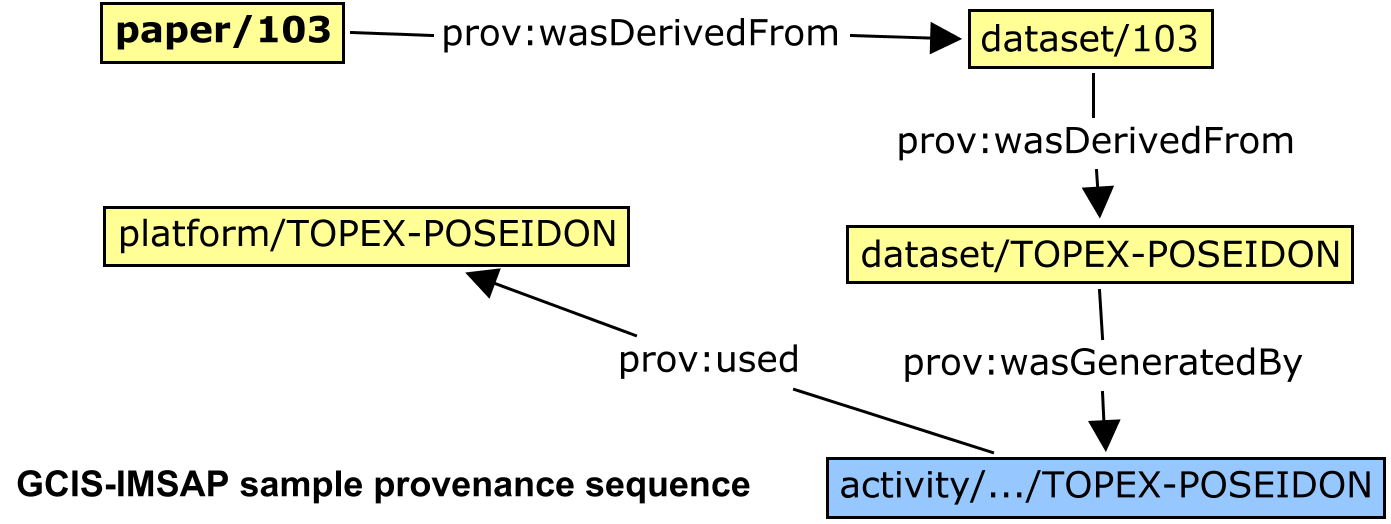
\includegraphics[width=\textwidth]{gcis-prov.png}
	\caption{Provenance graph fragment encoded in PROV-O}
	%\comment{to delete the caption inside the figure}
	\label{fig:gcis}
\end{figure}
The example is drawn from the Global Change Information System: Information Model and Semantic Application Prototypes (GCIS-IMSAP) project\footnote{Global Change Information System: Information Model and Semantic Application Prototypes: http://tw.rpi.edu/web/project/gcis-imsap}. The project models and captures provenance information for the recent National Climate Assessment (NCA) draft report\footnote{The full draft for public review is available at http://downloads.globalchange.gov/nca/nca3-drafts/NCAJan11-2013-publicreviewdraft-fulldraft.pdf} of the US Global Change Research Program (USGCRP).

From the provenance graph, we could get the information that the paper ``paper/103'' was derived from the dataset ``dataset/103'', which in turn was derived from the dataset ``dataset/TOPEX-POSEIDON'', which was generated by the activity ``activity/.../TOPEX-POSEIDON'' that used the platform ``platform/TOPEX-POSEIDON''. Irrelevant URI parts are omitted in the graph to make the meaning of the graph clear. Also note that all PROV-O properties use past tense verbs to emphasize that everything recorded in the provenance graph must be something that already happened.

Such information is quite useful for the general public to know the process of generating the reported results in the paper. However, for domain scientists who would like to verify the reported results or to base their new research on the work reported in this paper, the provenance graph is short on critical details such as:
\begin{itemize}
	\item How the reported results in ``paper/103'' were derived from ``dataset/103'', e.g., what data items were used to create a certain plot in the paper.
	\item How ``dataset/103'' was derived from ``dataset/TOPEX-POSEIDON'', e.g., what changes were made on what part of the original dataset to generate the derived one.
	\item How ``activity/.../TOPEX-POSEIDON'' used ``platform/TOPEX-POSEIDON'' to generate ``dataset/TOPEX-POSEIDON'', e.g., whether an algorithm and/or a model was used to deal with the raw data from the platform, what parameter values were used to run the algorithm and/or model.
\end{itemize} 
We define our provenance ontology for research publications, called PROV-PUB-O, by specializing the ``activity'' class and the ``used'' property in PROV-O to make the ontology suitable for capturing executable provenance in research publications.

Note that ``wasDerivedFrom'' do not need to be specialized because ``e1 wasDerivedFrom e2'' is a shortcut for ``a1 used e1; a1 generated e2'', where e1, e2 are PROV-O entities and a1 is an PROV-O activity. Neither do ``wasGeneratedBy'' since how an activity used its input entities already contains all the information needed for replicating the generation. The property ``wasGeneratedBy'' merely points out the output entity of the activity.

Interesting activities in the process of preparing research papers are all the changes of data, which can be classified into the following three categories:
\begin{itemize}
	\item Physical changes such as data download, copying, or sharing.
	\item Syntactical changes such as XML to JSON conversion.
	\item Semantic changes such as data analysis and transformation.
\end{itemize}
Each of the above changes corresponds to a certain way of data usage.

The specialized ontology is not only helpful in describing the provenance, but it also enables the construction of executable provenance graphs to preserve the data product preparing process at a level that is detailed enough to be replicable.

\begin{figure}
	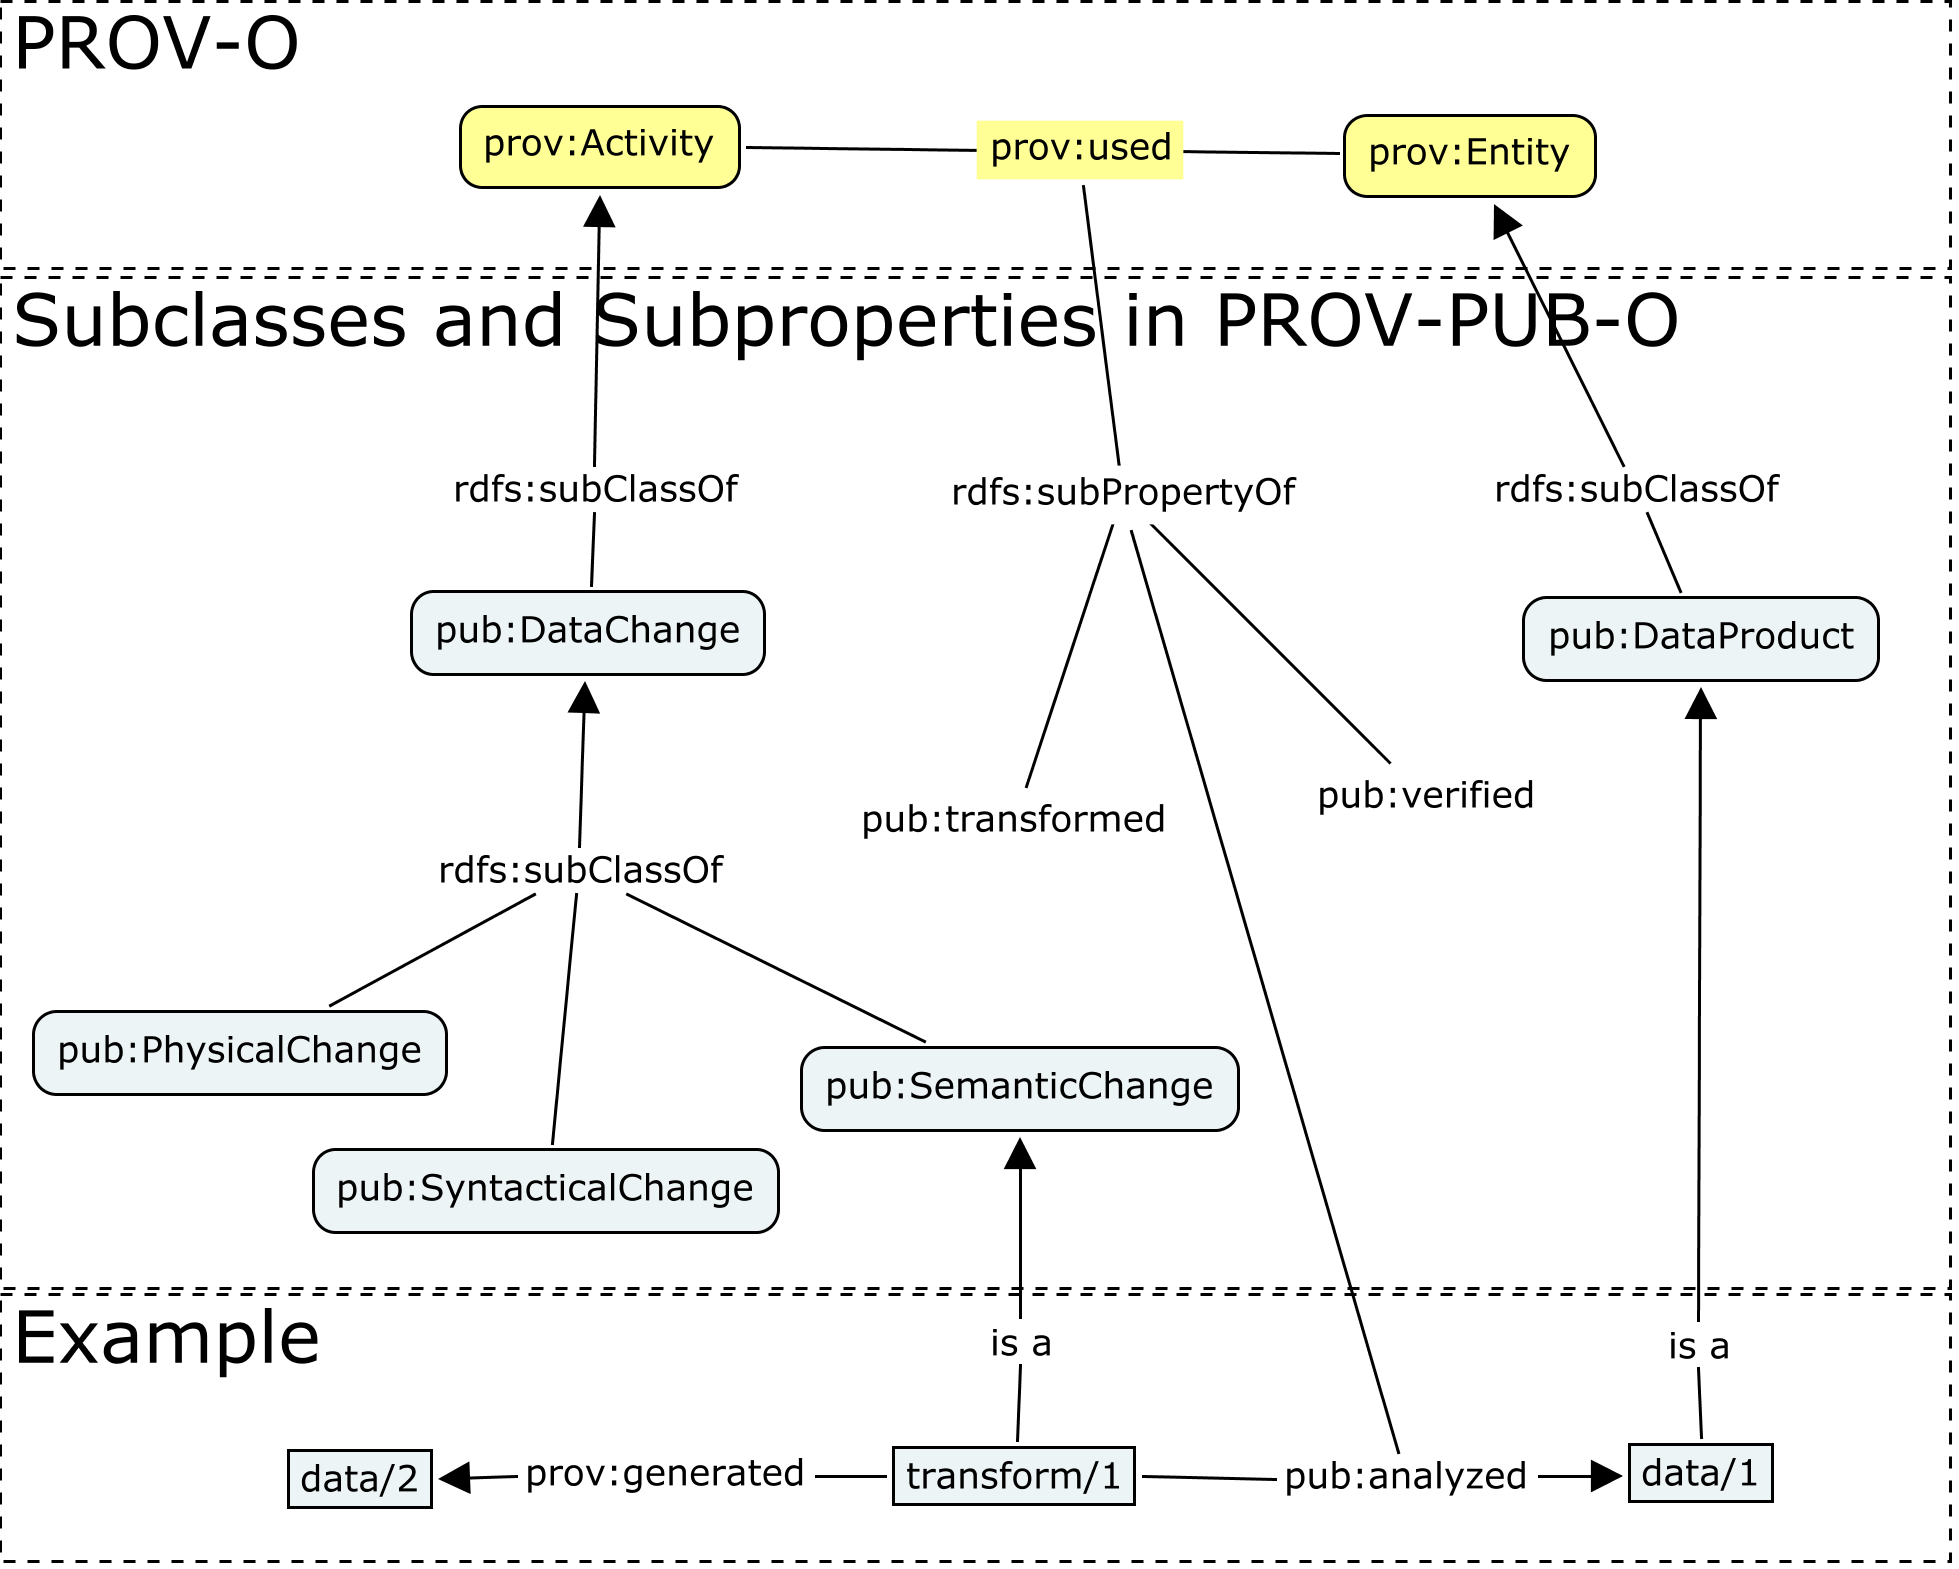
\includegraphics[width=\textwidth]{prov-pub-o.png}
	\caption{Illustrated sample provenance graph in PROV-PUB-O}
	%\comment{to replace this figure with a more developed one}
\end{figure}

The hypothesis we would like to justify here is that sub-properties of prov:used are more useful than prov:used itself in the use case of creating executable provenance graphs in the domain of earth science.

%\subsubsection{Workflow vs. provenance semantics}

%\subsubsection{Executable provenance graphs}

%\subsubsection{Ontology as software}

\subsection{Ontology usability evaluation approach}
\label{subsec:evaluation}
%\comment{We need to find a recurring scientific data analytics task as our use case. Then analyze the pros and cons of using general and specialized provenance ontologies.}

Nowadays many ontologies are written in Resource Description Framework Schema \cite{brickley2000resource} (RDFS) or Web Ontology Language \cite{mcguinness2004owl} (OWL). The evaluation of ontologies, however, has been paid attention to long before the introduction of these two ontology languages. For example, Gr{\"u}ninger et al in their paper \cite{gruninger1995methodology} proposes a method to check the completeness of an ontology with respect to a set of competency questions. Competency questions are the questions that the ontology is designed to answer, so this approach checks whether ``the right things are done''. Back then, ontologies are defined with first-order logic (or equivalently, in Knowledge Interchange Format (KIF)), so the authors formalized competency questions also with first-order logic and evaluate the ontology in question by proving completeness theorems with respect to these formal competency questions.

As more and more ontologies became available online (see Figure~\ref{fig:timeline} for a timeline of Semantic Web standards, and \cite{bikakis2013xml} for the details), attention is paid to the evaluation of ontologies for the purpose of selecting an existing ontology to reuse in a new application. A popular way to do this kind of evaluation is to define several criteria for decision making, evaluate the ontology in question on each of them, giving a numerical score, and compute the overall score for the ontology as a weighted sum of its per-criterion scores. This group of approaches is called \emph{multiple-criteria approaches} in \cite{brank2005survey}. For example, Fox et al in \cite{fox1995organisation} proposed a set of criteria including \emph{generality}, \emph{completeness}, \emph{perspicuity}, etc.; G{\'o}mez-P{\'e}rez in her paper \cite{gomez2001evaluation} published in 2001 pointed out the lack of interest in evaluation issues in the ontological engineering community at that time. She also pointed out that tools, tutorials and case studies are critical for ontology engineers to assess the usability of an existing ontology. Unfortunately the paper does not give an example of ontology usability evaluation, it instead evaluates the Standard-Unit Ontology in terms of consistency, completeness and conciseness; Lozano-Tello et al present the \emph{ONTOMETRIC} method \cite{lozano2003selection,lozano2004ontometric}, which compares ontologies with a taxonomy of
160 characteristics organized in a multilevel framework. At the top level, there are five basic aspects. These are: the \emph{content} of the ontology and the
organization of their contents, the \emph{language}
in which it is implemented, the \emph{methodology}
that has been followed to develop it,
the software \emph{tools} used to build and edit
the ontology, and the \emph{costs} that the ontology
will be necessary in a certain project. For each ontology under consideration, the ONTOMETRIC method basically calculates the weighted sum of the scores given to each of the leaf node characteristics of this tree-shaped framework. Aggregated scores are obtained for sub-tree roots as the calculation ascending each level along the tree, so the final score is finally available at the root node. Hartmann et al in \cite{hartmann2005d1} pointed out the following two usability issues of ONTOMETRIC:
\begin{itemize}
	\item Specifying the characteristics of an ontology
	is complicated and takes time
	\item Assessing
	the characteristics is quite subjective (from the
	project managers' viewpoint)
\end{itemize} 

\begin{figure}
	\centering
	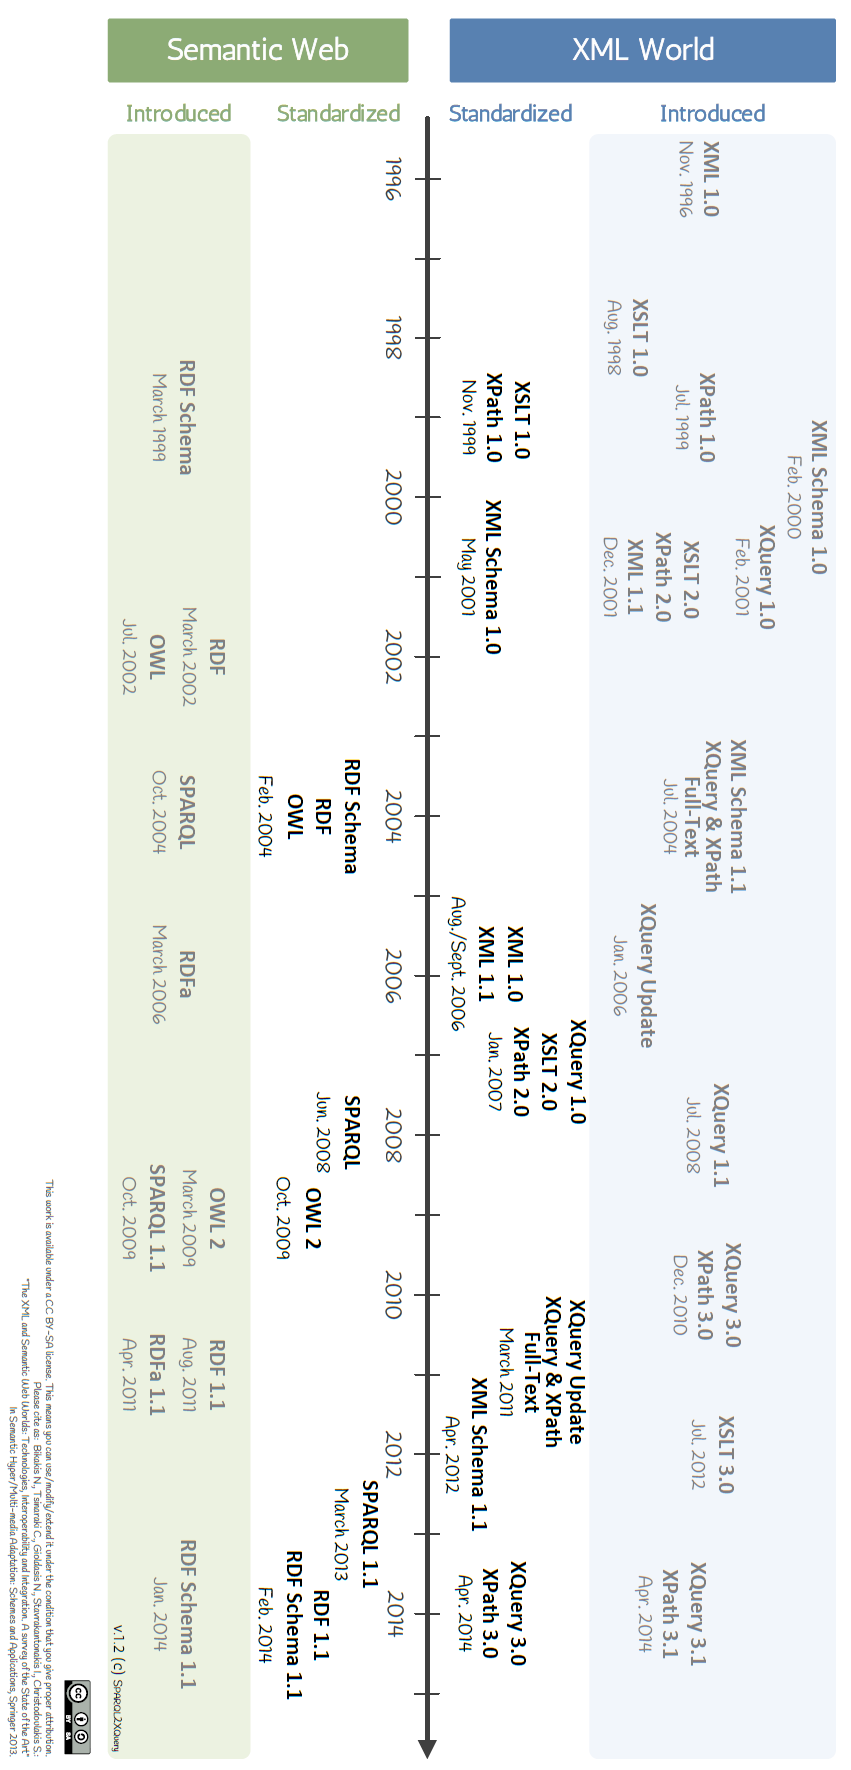
\includegraphics[width=\linewidth]{XMLSemanticWebW3CTimeline}
	\caption[XML and Semantic Web W3C Standards Timeline]{XML and Semantic Web W3C Standards Timeline}
	\label{fig:timeline}
\end{figure}

Different from the studies mentioned above, Burton-Jones et al proposed a set of 10 objective metrics at 4 different levels of a semiotic framework in \cite{burton2005semiotic}. Their work supports objective evaluation of ontologies, which does not require experts' review of the ontologies in questions. 

In \cite{gangemi2006qood}, Gangemi et al organized the criteria for ontology evaluation and selection with a semiotic meta-ontology called $O^2$ and the \emph{oQual} evaluation ontology which involves concepts and relations relevant to ontology evaluation and selection. Therefore, evaluation based on the oQual ontology goes beyond the mere calculation of a weighted sum, but also contains reasoning based on the evaluation ontology. 
%\comment{to read: OntoQA \cite{tartir2005ontoqa} (schema- and instance- level metrics) Ontology metrics design \cite{vrandevcic2007design} Unit tests for ontologies \cite{vrandevcic2006unit}.} 

However, few of these studies deal with the usability evaluation of ontologies. 

The few work dealing with ontology usability evaluation includes \cite{casellas2009ontology}, which used System Usability Scale \cite{brooke1996sus} to evaluate the usability of the Ontology of Professional Judicial Knowledge (See Chapter 2 of \cite{casellas2009ontology} for a good introduction of the ontology).

We propose an objective evaluation measurement based on the Halstead complexity measures (\cite{halstead1977elements}, paraphrased in \cite{weyuker1988evaluating}), and we choose the task of data preparation for our evaluation. Data preparation loosely means indexing, organizing and optimizing data so they become structured in a form that 1) people can use and 2) software can consume. Figure~\ref{fig:data-analytics} shows how data preparation is related to other data analytics tasks\footnote{http://tw.rpi.edu/media/latest/DataAnalytics2015\_week1a.ppt [Retrived on May 11th, 2015]}. It is also called data munging and a sense of it could be obtained via reading any textbook talking about a data processing oriented programming language such as Perl \cite{cross2001data}.

\begin{figure}
	\centering
	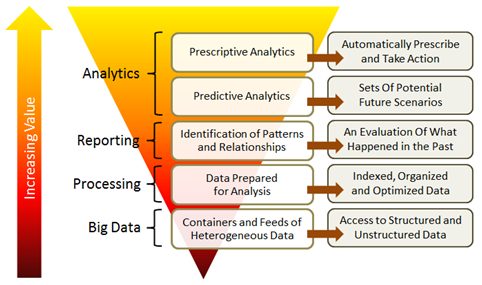
\includegraphics[width=\linewidth]{data-analytics.png}
	\caption{Data analytics levels}
	\label{fig:data-analytics}
\end{figure}

The basic idea is: provenance ontologies are used in software tools capturing provenance and reproducing the process of a certain task such as data preparation, so to evaluate the usability of such ontologies, we look at the complexity of software tools built on them. The less complex the software, the more usable the ontology.

\begin{itemize}
\item $\eta_1 = $Number of distinct operators.
\item $\eta_2 = $Number of distinct operands.
\item $N_1 = $Total number of operators.
\item $N_2 = $Total number of operands.
\end{itemize}
%The program volume is defined to be
%\begin{equation}
%V = (N_1+N_2) \log_2(\eta_1+\eta_2).
%\end{equation}
An approximate formula for programming effort as a measure of program complexity is:
\begin{equation}
E = \frac{\eta_1N_2(N_1+N_2)\log_2(\eta_1+\eta_2)}{2\eta_2}.
\end{equation}

We choose the Halstead measure because the comparison of programming on top of different ontologies is mostly about the number and types of operations, rather than data flows (e.g., Oviedo in \cite{oviedo1993control} proposed a measure based on program data flows).

We draw our data preparing operations from the R programming language. The assumption is that R is a data processing oriented programming language and the operations covered by R are typical for data processing.

So the operations we are looking at are:
\begin{itemize}
	\item importing data from a file (be it a text file, an Excel spreadsheet, an XML file, or a netCDF file),
	\item webscraping,
	\item annotating datasets,
	\item combining objects into a vector,
	\item combining objects as columns or rows.
\end{itemize}

Currently we are picking typical data preparation tasks and describing them as combinations of the operations mentioned above. The plan is to calculate Halstead complexity values for programs based on PROV-PUB-O and directly on PROV-O for each hypothesis listed in the previous subsection to validate it.

We originally planned to also describe the automatic provenance capturing mechanism and the proof-of-concept platform in this chapter. But the PROV-PUB-O part expands unexpectedly well and we decided to focus on it and move the other two sections to the future work chapter.

%\resetfootnote %this command starts footnote numbering with 1 again.

%\begin{figure}
%\centering
%\vspace{2.0in}
%\caption[A Shorter Caption for the List of Figures]
%   {This is the Caption for the First Figure in Chapter 2.  It is a
%    long, long caption; we do not want to put the whole thing in the
%    List of Figures. A Shorter Caption can go in the square brackets.}
% If you like additional lines in the caption indented, see the root template
% file rpithes.tex for an example of using the caption package to do this.
%\end{figure}
 
%This is shown in table~\ref{mytable}.  % see \label below
 
%\begin{table}
%\caption{This is the Caption for Table 2}
%\label{mytable}        % \label command must always comes AFTER the caption
%\begin{center}
%\begin{tabular}{lll}
%Here's       & another     & example  \\
%of           & a           & table    \\
%floated      & with        & the      \\
%\verb+table+ & environment & command.
%\end{tabular}
%\end{center}
%\end{table}


%\section{This is a Section Heading}
 
%\subsection{This is a Subsection Heading} 
 
%Text before a footnote.\footnote{Here's the text of the footnote.}
%Text after the footnote.


%%% Local Variables: 
%%% mode: latex
%%% TeX-master: t
%%% End: 
